\documentclass[12pt]{article}
\usepackage{hyperref,amsmath,amsfonts,amssymb,fullpage,color}
\usepackage{enumitem}
\usepackage{tikz}
\newcommand{\be}{\begin{equation}}
\newcommand{\ee}{\end{equation}}
\newcommand{\bh}{\bar{h}}
\newcounter{quesno}
\newcommand{\ques}[1]{\vspace{2em}\stepcounter{quesno}
\noindent{\bf Question \thequesno.} \emph{(#1 points)\\}
}
\begin{document}

\begin{center}
{\bf\Large General Relativity}

\vspace{1em}
{\bf\large Final Examination --- Answers}
\end{center}

\vspace{1em}
\hrule

% ---------------------------------------------------------------- Q1
\ques{2}
\textbf{Transformation law.} Under a change of coordinates $x^\mu \to x'^\mu(x)$ the Riemann tensor, a $(1,3)$ tensor, transforms as
\be
R'^{\mu}{}_{\nu\rho\sigma}
= \frac{\partial x'^\mu}{\partial x^\alpha}\,
  \frac{\partial x^\beta}{\partial x'^\nu}\,
  \frac{\partial x^\gamma}{\partial x'^\rho}\,
  \frac{\partial x^\delta}{\partial x'^\sigma}\;
  R^{\alpha}{}_{\beta\gamma\delta}\,.
\ee

\textbf{Ricci tensor.} By definition $R'_{\mu\nu} = R'^{\rho}{}_{\mu\rho\nu}$. Inserting the law above (upper index $\to\rho$, and the third index set equal to $\rho$):
\be
R'_{\mu\nu} = R'^{\rho}{}_{\mu\rho\nu}
= \frac{\partial x'^\rho}{\partial x^\alpha}\,
  \frac{\partial x^\beta}{\partial x'^\mu}\,
  \frac{\partial x^\gamma}{\partial x'^\rho}\,
  \frac{\partial x^\delta}{\partial x'^\nu}\;
  R^{\alpha}{}_{\beta\gamma\delta}\,.
\ee
The sum over $\rho$ involves only the two Jacobians $\frac{\partial x'^\rho}{\partial x^\alpha}\frac{\partial x^\gamma}{\partial x'^\rho}$, and by the chain rule
\be
\frac{\partial x^\gamma}{\partial x'^\rho}\frac{\partial x'^\rho}{\partial x^\alpha}
= \frac{\partial x^\gamma}{\partial x^\alpha} = \delta^\gamma_\alpha\,.
\ee
Therefore
\be
R'_{\mu\nu}
= \frac{\partial x^\beta}{\partial x'^\mu}\,
  \frac{\partial x^\delta}{\partial x'^\nu}\;
  \delta^\gamma_\alpha R^{\alpha}{}_{\beta\gamma\delta}
= \frac{\partial x^\beta}{\partial x'^\mu}\,
  \frac{\partial x^\delta}{\partial x'^\nu}\; R^{\alpha}{}_{\beta\alpha\delta}
= \frac{\partial x^\beta}{\partial x'^\mu}\,
  \frac{\partial x^\delta}{\partial x'^\nu}\; R_{\beta\delta}\,,
\ee
which is precisely the transformation law of a $(0,2)$ tensor. $\qquad\blacksquare$

% ---------------------------------------------------------------- Q2
\ques{3}
Write $\hat\Gamma_{\mu\nu}{}^\rho = \Gamma_{\mu\nu}{}^\rho + K_{\mu\nu}{}^\rho$ with $K_{\mu\nu}{}^\rho = \frac{1}{12}g^{\rho\sigma}H_{\mu\nu\sigma}$, so that $K_{\mu\nu\sigma} = \frac1{12}H_{\mu\nu\sigma}$ is totally antisymmetric. (The difference of two connections is a tensor, so this is a legitimate connection.)

\begin{enumerate}[label=\alph*)]
\item \textbf{Torsion.} The Levi-Civita connection is symmetric, $\Gamma_{\mu\nu}{}^\rho=\Gamma_{\nu\mu}{}^\rho$, so the torsion is
\be
\hat T_{\mu\nu}{}^\rho = \hat\Gamma_{\mu\nu}{}^\rho - \hat\Gamma_{\nu\mu}{}^\rho
= K_{\mu\nu}{}^\rho - K_{\nu\mu}{}^\rho = \frac{1}{12}g^{\rho\sigma}\left(H_{\mu\nu\sigma}-H_{\nu\mu\sigma}\right)
= \frac{1}{6}\,g^{\rho\sigma}H_{\mu\nu\sigma}\,.
\ee
This is non-zero whenever $H\neq0$, so $\hat\Gamma$ is \emph{not} torsion-free (it is torsion-free only if $H=0$).

\textbf{Metric compatibility.} Since the Levi-Civita part satisfies $\nabla_\sigma g_{\mu\nu}=0$,
\be
\hat\nabla_\sigma g_{\mu\nu} = \nabla_\sigma g_{\mu\nu} - K_{\sigma\mu}{}^\lambda g_{\lambda\nu} - K_{\sigma\nu}{}^\lambda g_{\mu\lambda}
= -K_{\sigma\mu\nu} - K_{\sigma\nu\mu} = -\frac{1}{12}\left(H_{\sigma\mu\nu}+H_{\sigma\nu\mu}\right) = 0\,,
\ee
by the antisymmetry of $H$ in its last two indices. (Because $H$ is totally antisymmetric the result is the same whichever of the first two indices of $\hat\Gamma$ is taken as the derivative index.) So $\hat\Gamma$ \emph{is} metric compatible.

\item The geodesic equation for $\hat\Gamma$ is
\be
\frac{d^2x^\rho}{d\tau^2} + \hat\Gamma_{\mu\nu}{}^\rho\frac{dx^\mu}{d\tau}\frac{dx^\nu}{d\tau}=0
\quad\Longleftrightarrow\quad
\frac{d^2x^\rho}{d\tau^2} + \Gamma_{\mu\nu}{}^\rho\frac{dx^\mu}{d\tau}\frac{dx^\nu}{d\tau}
+ \frac{1}{12}g^{\rho\sigma}H_{\mu\nu\sigma}\frac{dx^\mu}{d\tau}\frac{dx^\nu}{d\tau}=0\,.
\ee
The last term contracts the symmetric object $\dot x^\mu\dot x^\nu$ with $H_{\mu\nu\sigma}$, which is antisymmetric in $\mu\nu$, so it vanishes identically. The equation reduces to the Levi-Civita geodesic equation (with the same affine parameter), so the geodesics coincide. (Only the symmetric part of a connection matters for geodesics; the torsion drops out.)
\end{enumerate}

% ---------------------------------------------------------------- Q3
\ques{4}
\begin{enumerate}[label=\alph*)]
\item The metric components are singular at $r=0$, at $r=2GM$ and (trivially) at $\theta=0,\pi$. The latter are just the usual coordinate singularities of spherical polar coordinates (the same as the poles of a globe), removed by going to Cartesian-like coordinates.

\begin{itemize}
\item $r=2GM$ (the event horizon), where $g_{tt}\to0$ and $g_{rr}\to\infty$, is a \emph{coordinate singularity}: it is a failure of the $(t,r)$ coordinates, not of the geometry. All curvature invariants are finite there; e.g.\ the Kretschmann scalar is
\be
R_{\mu\nu\rho\sigma}R^{\mu\nu\rho\sigma} = \frac{48\,G^2M^2}{r^6}\,\xrightarrow{r=2GM}\, \frac{3}{4G^4M^4}<\infty,
\ee
and a freely falling observer crosses it in finite proper time and feels nothing special (tidal forces $\sim GM/r^3$ are finite and small for a large black hole).
\item $r=0$ is a genuine \emph{curvature singularity}: $R_{\mu\nu\rho\sigma}R^{\mu\nu\rho\sigma}=48G^2M^2/r^6\to\infty$, which is a coordinate-independent statement. Tidal forces diverge, and every infalling observer reaches it in finite proper time (at most $\pi GM$ for radial infall from the horizon) where geodesics end. This is what one should be concerned about.
\end{itemize}
(The horizon is still one-way: once inside, one cannot return, but that is not a singularity of the metric.)

\item Define $r_*=r+2GM\ln|r/2GM-1|$, so $v=t+r_*$. Then
\be
\frac{dr_*}{dr}=1+\frac{2GM}{r-2GM}=\frac{r}{r-2GM}=\frac1{f(r)}\,,
\qquad dv = dt+\frac{dr}{f}\;\Rightarrow\; dt = dv-\frac{dr}{f}\,.
\ee
Substituting,
\be
-f\,dt^2 = -f\left(dv^2-\frac{2}{f}dv\,dr+\frac{dr^2}{f^2}\right)=-f\,dv^2+2\,dv\,dr-\frac{dr^2}{f}\,,
\ee
and adding $f^{-1}dr^2$ the $dr^2$ terms cancel:
\be
ds^2 = -\left(1-\frac{2GM}{r}\right)dv^2 + 2\,dv\,dr + r^2\left(d\theta^2+\sin^2\theta\,d\phi^2\right).
\ee
\textbf{Interpretation.} In the $(v,r)$ block the metric is $\begin{pmatrix}-f&1\\1&0\end{pmatrix}$ with determinant $-1$: it is finite, smooth and invertible at $r=2GM$ (all components are analytic there, and the inverse metric is regular too). Thus $r=2GM$ is only a coordinate artefact of $(t,r)$, and the spacetime extends smoothly through it into $r<2GM$. In these coordinates the radial null rays satisfy $dv(-f\,dv+2\,dr)=0$: ingoing rays are $v=$ const, and the other family has $dr/dv=f/2$, which for $r<2GM$ is negative, so that \emph{all} future light cones point towards decreasing $r$ and nothing escapes. The only place where the metric genuinely misbehaves is $r=0$ ($f\to\infty$), consistent with the curvature singularity found in a). Hence one can fall through $r=2GM$ safely but not avoid $r=0$.
\end{enumerate}

% ---------------------------------------------------------------- Q4
\ques{5}
\begin{enumerate}[label=\alph*)]
\item The metric has the Friedmann--Lema\^{i}tre--Robertson--Walker form
\be
ds^2=-dt^2+a(t)^2\,d\Omega_3^2\,,\qquad d\Omega_3^2=d\chi^2+\sin^2\chi\,d\Omega_2^2\,,
\ee
with spatial slices that are round three-spheres ($k=+1$). Spatial slices are homogeneous and isotropic, as the cosmological principle and the observed large-scale uniformity (and the CMB isotropy) require. The \textbf{scale factor} is
\be
a(t)=L\cosh(t/L)\,.
\ee
It is a solution of the Einstein equations with a positive cosmological constant: with $\dot a=\sinh(t/L)$,
\be
H^2+\frac{k}{a^2}=\frac{\dot a^2+1}{a^2}=\frac{\cosh^2(t/L)}{L^2\cosh^2(t/L)}=\frac1{L^2}=\frac{\Lambda}{3}\,,\qquad \Lambda=\frac{3}{L^2},
\ee
which is the Friedmann equation for vacuum energy only. At late times $a\simeq\frac L2e^{t/L}$: exponential, accelerating expansion, as seen in our universe at present (dark energy) and as in inflation. It is a good model of a $\Lambda$-dominated universe, although an exactly empty one is only an approximation to ours.

\item Suppose $g_{\mu\nu}=\Omega^2\bar g_{\mu\nu}$ with $\Omega$ smooth and nowhere zero. For any vector $V$, $g(V,V)=\Omega^2\,\bar g(V,V)$, so $g(V,V)$ and $\bar g(V,V)$ have the same sign: timelike, null and spacelike vectors and curves are the same in both metrics. In particular, the light cones are identical (null curves $ds^2=0$ coincide, $\Omega^2\bar g=0\Leftrightarrow\bar g=0$), and so are the notions of causal curves, time orientation, and causal past and future. Causal structure depends only on the light-cone structure, hence is the same. (Distances and proper times differ, but they are not part of the causal structure.)

\item With $\cosh(t/L)=1/\cos\eta$ and $t\in(-\infty,\infty)$ we get $\eta\in(-\pi/2,\pi/2)$, and $\sinh(t/L)=\sqrt{\cosh^2-1}=\tan\eta$ (same sign as $t$). Differentiating,
\be
\frac1L\sinh(t/L)\,dt=\frac{\sin\eta}{\cos^2\eta}\,d\eta
\;\Rightarrow\; dt=\frac{L\,d\eta}{\cos\eta}\,.
\ee
Therefore
\be
ds^2=\frac{L^2}{\cos^2\eta}\left[-d\eta^2+d\chi^2+\sin^2\chi\left(d\theta^2+\sin^2\theta\,d\phi^2\right)\right],
\ee
which is conformal (with $\Omega=L/\cos\eta$) to the Einstein static universe $\mathbb R\times S^3$ restricted to the finite strip $-\pi/2<\eta<\pi/2$, $0\le\chi\le\pi$. By b), de Sitter therefore has the same causal structure as this finite region of the Einstein static universe, and radial null rays obey $d\eta=\pm d\chi$, i.e.\ are straight lines at $45^\circ$ in the $(\chi,\eta)$ plane.

\emph{Penrose diagram.} It is a square of width $\pi$ (in $\chi$) and height $\pi$ (in $\eta$), each point representing a two-sphere of radius $L\sin\chi/\cos\eta$:
\begin{itemize}
\item the left edge $\chi=0$ and the right edge $\chi=\pi$ are the north and south poles of the $S^3$: these are \emph{not} boundaries but lines of origin, along which the sphere shrinks to zero size (timelike worldlines of observers at the poles);
\item the top edge $\eta=\pi/2$ is future infinity $\mathcal I^+$ ($t\to\infty$) and the bottom edge $\eta=-\pi/2$ is past infinity $\mathcal I^-$ ($t\to-\infty$); both are \emph{spacelike};
\item the horizontal line $\eta=0$ is the moment of time symmetry $t=0$, where the $S^3$ has its minimum radius $L$ (the universe contracts for $t<0$ and expands for $t>0$).
\end{itemize}

\begin{center}
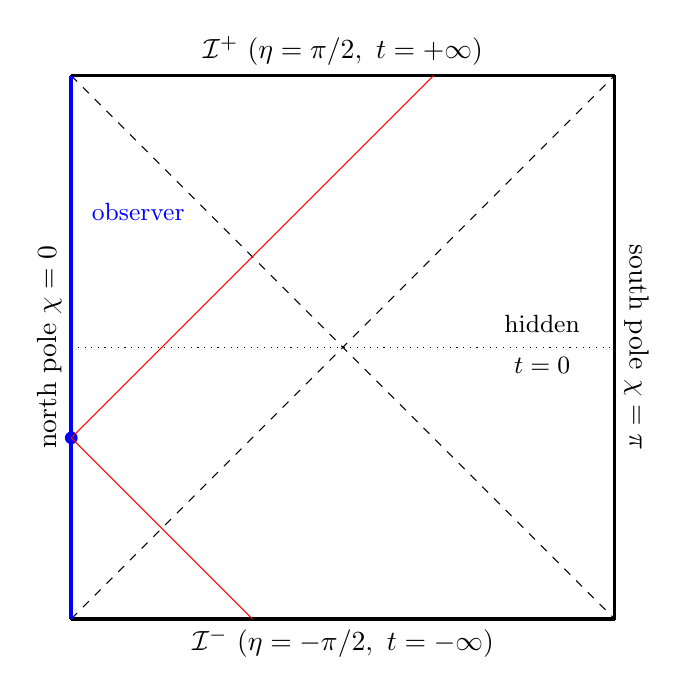
\begin{tikzpicture}[scale=1.15]
% square
\draw[thick] (0,0) rectangle (6,6);
% scri
\draw[very thick] (0,6) -- (6,6);
\draw[very thick] (0,0) -- (6,0);
\node[above] at (3,6) {$\mathcal I^+\ (\eta=\pi/2,\ t=+\infty)$};
\node[below] at (3,0) {$\mathcal I^-\ (\eta=-\pi/2,\ t=-\infty)$};
\node[left,rotate=90,anchor=south] at (0,3) {north pole $\chi=0$};
\node[right,rotate=-90,anchor=south] at (6,3) {south pole $\chi=\pi$};
% t=0 slice
\draw[dotted] (0,3) -- (6,3) node[right] {};
\node[below] at (5.2,3) {\small $t=0$};
% diagonals
\draw[dashed] (0,0) -- (6,6);
\draw[dashed] (0,6) -- (6,0);
% observer at the north pole
\draw[ultra thick,blue] (0,0) -- (0,6);
\fill[blue] (0,2) circle (2pt);
% past and future light cone of the point (0,2)
\draw[red,thin] (0,2) -- (4,6);
\draw[red,thin] (0,2) -- (2,0);
% ends of the observer worldline
\node[blue,anchor=west] at (0.12,4.5) {\small observer};
\node[above] at (5.2,3.05) {\small hidden};
\end{tikzpicture}
\end{center}
The dashed diagonals are the horizons of the observer on the left edge, whose worldline ends at the top-left corner. The diagonal from top-left to bottom-right is the boundary of the observer's causal past, the \emph{event horizon}: signals emitted from the region above it (labelled ``hidden'') can never reach the observer, and it is also the limit of the observer's past light cone (the particle horizon) as $t\to\infty$; at any finite time the observer sees only a smaller region (the red past light cone is an example). The diagonal from bottom-left to top-right is the boundary of the causal future of the observer's worldline: the observer can never influence events below it. A light ray from one pole reaches the opposite pole only at a corner of the diagram, i.e.\ at $\mathcal I^\pm$. Hence the de Sitter Penrose diagram is a square with spacelike $\mathcal I^\pm$ and horizons for every geodesic observer.
\end{enumerate}

% ---------------------------------------------------------------- Q5
\ques{6}
\begin{enumerate}[label=\alph*)]
\item Linearised diffeomorphisms $x^\mu\to x^\mu+\xi^\mu$ act as $h_{\mu\nu}\to h_{\mu\nu}-\partial_\mu\xi_\nu-\partial_\nu\xi_\mu$, so
\be
\bh_{\mu\nu}\to\bh_{\mu\nu}-\partial_\mu\xi_\nu-\partial_\nu\xi_\mu+\eta_{\mu\nu}\partial_\rho\xi^\rho\,,\qquad
\partial^\mu\bh_{\mu\nu}\to\partial^\mu\bh_{\mu\nu}-\partial^\rho\partial_\rho\xi_\nu\,.
\ee
Choosing $\xi_\nu$ to solve $\partial^\rho\partial_\rho\xi_\nu=\partial^\mu\bh_{\mu\nu}$ (always possible: this is a wave equation with a source) imposes the Lorenz (de Donder) gauge $\partial^\mu\bh_{\mu\nu}=0$. Then the second and third terms of the equation vanish and
\be
-\frac12\,\partial^\rho\partial_\rho\,\bh_{\mu\nu}=8\pi G\,T_{\mu\nu}\quad\Longleftrightarrow\quad
\left(-\partial_t^2+\nabla^2\right)\bh_{\mu\nu}=-16\pi G\,T_{\mu\nu}\,.
\ee
In vacuum this is the wave equation $\Box\bh_{\mu\nu}=0$: the perturbations propagate at the speed of light as \emph{gravitational waves}, $\bh_{\mu\nu}=A_{\mu\nu}e^{ik\cdot x}$ with $k^\mu k_\mu=0$ and $k^\mu A_{\mu\nu}=0$. (The residual gauge freedom $\Box\xi=0$ can be used to reach the transverse-traceless gauge, leaving two physical polarisations, $+$ and $\times$.)

\item The perturbation has $h_{0\mu}=0$ (TT gauge). The geodesic equation for a particle initially at rest, $u^\mu=(1,0,0,0)$, has
\be
\frac{d^2x^i}{d\tau^2}=-\Gamma^i_{00}=-\frac12\eta^{ij}\left(2\partial_0h_{j0}-\partial_jh_{00}\right)=0\,.
\ee
Hence the free particles stay at \emph{fixed coordinate positions}: coordinates are comoving with the test masses, and the wave shows up only as a change in the metric components.

At fixed time $t$ the spatial metric is $g_{xx}=1+h_+(t-z)$, $g_{yy}=1-h_+(t-z)$, $g_{zz}=1$ (and $|h_+|\ll1$). The two particles on the $x$-axis both have $y=z=0$, so $h_+(t-z)=h_+(t)$ everywhere on the segment joining them, and
\be
\Delta s=\int_0^{L_x}\sqrt{g_{xx}}\,dx=\int_0^{L_x}\sqrt{1+h_+(t)}\,dx=L_x\sqrt{1+h_+(t)}\approx L_x\left(1+\frac12h_+(t)\right).
\ee
For the third particle at $(0,L_y,0)$, the segment lies along $y$ at $x=z=0$:
\be
\Delta s=\int_0^{L_y}\sqrt{g_{yy}}\,dy=L_y\sqrt{1-h_+(t)}\approx L_y\left(1-\frac12h_+(t)\right).
\ee
So the wave alternately stretches the $x$-separation and squeezes the $y$-separation, and vice versa half a period later, with a \emph{differential} strain $(\Delta s_x/L_x)-(\Delta s_y/L_y)=h_+(t)$.

\item \textbf{Qualitative picture.} Two masses $m_1,m_2$ in orbit have a time-dependent mass quadrupole moment, which radiates gravitational waves (there is no monopole or dipole radiation by conservation of mass and momentum). The waves have frequency twice the orbital frequency, $f_{\rm GW}=2f_{\rm orb}$, and carry away energy and angular momentum. The orbit therefore shrinks, the bodies orbit faster, and the radiation becomes stronger---a runaway process that ends in a merger. (This was confirmed indirectly by the decay of the Hulse--Taylor binary pulsar orbit.) Three phases:

\begin{itemize}
\item \emph{Inspiral:} the separation shrinks slowly and adiabatically, quasi-circular orbits with increasing frequency and amplitude, so the signal is a \emph{chirp}. At leading order
\be
f_{\rm GW}\propto(t_c-t)^{-3/8},\qquad h\propto\frac{(G\mathcal M_c)^{5/3}f^{2/3}}{c^4\,d}\,,\qquad \mathcal M_c=\frac{(m_1m_2)^{3/5}}{(m_1+m_2)^{1/5}}\,,
\ee
where $d$ is the distance to the source and $t_c$ the coalescence time. The rate at which the frequency sweeps up measures the chirp mass $\mathcal M_c$, the amplitude then gives the distance $d$, and subtle higher-order effects encode the mass ratio and spins.
\item \emph{Merger:} when the separation reaches roughly the innermost stable circular orbit, $r\sim6GM/c^2$ (at $f_{\rm GW}\sim c^3/(6^{3/2}\pi GM)\approx4.4\,{\rm kHz}\,(M_\odot/M)$), the bodies plunge together and merge into a single, highly distorted black hole. The signal reaches maximum amplitude and frequency; the dynamics is strongly non-linear and strongly curved, and is accessible only through numerical relativity. A few per cent of the total rest mass is radiated in the last few cycles (about $3M_\odot c^2$ in GW150914).
\item \emph{Ringdown:} the remnant black hole radiates away its deformations as a superposition of damped sinusoids (quasi-normal modes), $h\sim e^{-t/\tau}\cos(2\pi f_{\rm qnm}t)$, and settles to a stationary Kerr black hole. The frequency and decay time depend only on the final mass and spin (no-hair theorem), so the ringdown tests general relativity and measures the remnant's properties.
\end{itemize}

\begin{center}
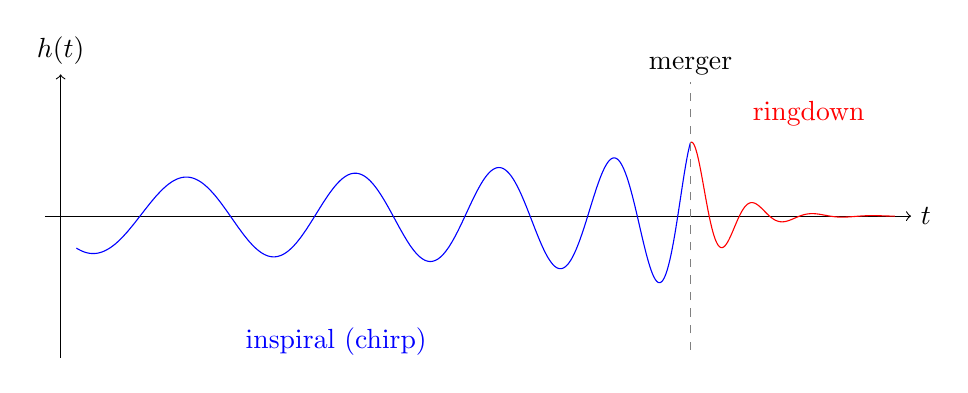
\begin{tikzpicture}[scale=1.0]
\draw[->] (-0.2,0) -- (10.8,0) node[right] {$t$};
\draw[->] (0,-1.8) -- (0,1.8) node[above] {$h(t)$};
% inspiral
\draw[blue,samples=700,smooth,domain=0.2:8.0]
  plot ({\x},{1.0*0.8*(8.4-\x)^(-0.25)*sin((-9.0*(8.4-\x)^(0.625)) r)});
% ringdown
\draw[red,samples=300,smooth,domain=8.0:10.6]
  plot ({\x},{1.0*exp(-(\x-8.0)/0.45)*sin((-5.08+8.2*(\x-8.0)) r)});
\draw[dashed,gray] (8.0,-1.7) -- (8.0,1.7);
\node[blue] at (3.5,-1.6) {inspiral (chirp)};
\node at (8.0,1.9) {merger};
\node[red] at (9.5,1.3) {ringdown};
\end{tikzpicture}
\end{center}
The amplitude and frequency both rise through the inspiral, peak at merger, and then the signal decays exponentially at a nearly constant frequency.

\textbf{Interferometric detection.} A detector such as LIGO is a Michelson interferometer with two perpendicular arms, each of length $L\approx4\,$km (made effectively longer, $\sim1000$\,km, by Fabry--P\'erot cavities), with suspended mirrors acting as free test masses (they are free to move horizontally for frequencies above the pendulum frequency). A laser beam is split at a beam splitter, travels down both arms, reflects, and recombines at a photodetector; the arm lengths are tuned so that, without a wave, the light interferes destructively at the output (a \emph{dark fringe}). By part b), a $+$ polarised wave incident from above, with the arms along $x$ and $y$, stretches one arm and shrinks the other: $\Delta L_x=+\frac12Lh_+$, $\Delta L_y=-\frac12Lh_+$, so the \emph{differential} arm-length change is $\Delta L_x-\Delta L_y=L\,h_+(t)$. This changes the round-trip light travel times and so the relative phase of the two beams, $\Delta\phi\simeq 4\pi L\,h_+/\lambda$ (for a single round trip), and the light power at the photodetector varies in proportion to $h(t)$. The detector therefore records the wave strain directly as a time series: $h\sim10^{-21}$ means $\Delta L\sim10^{-18}$\,m, far smaller than a proton, and this requires great isolation from noise. (A $\times$ polarised wave stretches along the diagonals; arbitrary sources give $h=F_+h_++F_\times h_\times$ with antenna factors $F_{+,\times}$, so several detectors are needed to localise a source.)

\textbf{Connecting signal to physics.} Frequency evolution during inspiral gives $\mathcal M_c$; the amplitude then gives the distance; the merger frequency, $\propto1/M$, gives the total mass; the ringdown frequency and damping time give the final mass and spin; the ratio of the $+$ and $\times$ amplitudes tells the inclination of the orbital plane; and the total radiated energy is the difference between the initial total mass and the final mass.
\end{enumerate}

\end{document}
